\chapter{Introduction and motivation}

Cell membrane represents an interface between the cell and its external environment. The first mention of the idea that cells are surrounded by a thin layer called a plasma membrane goes back to the second half of the 19$^{\text{th}}$ century. Over the years the structure and biophysical properties of the cell membrane have been extensively investigated and nowadays they are well defined and described \cite{Edidin2003}.

\begin{figure}[!ht]
\begin{center}
 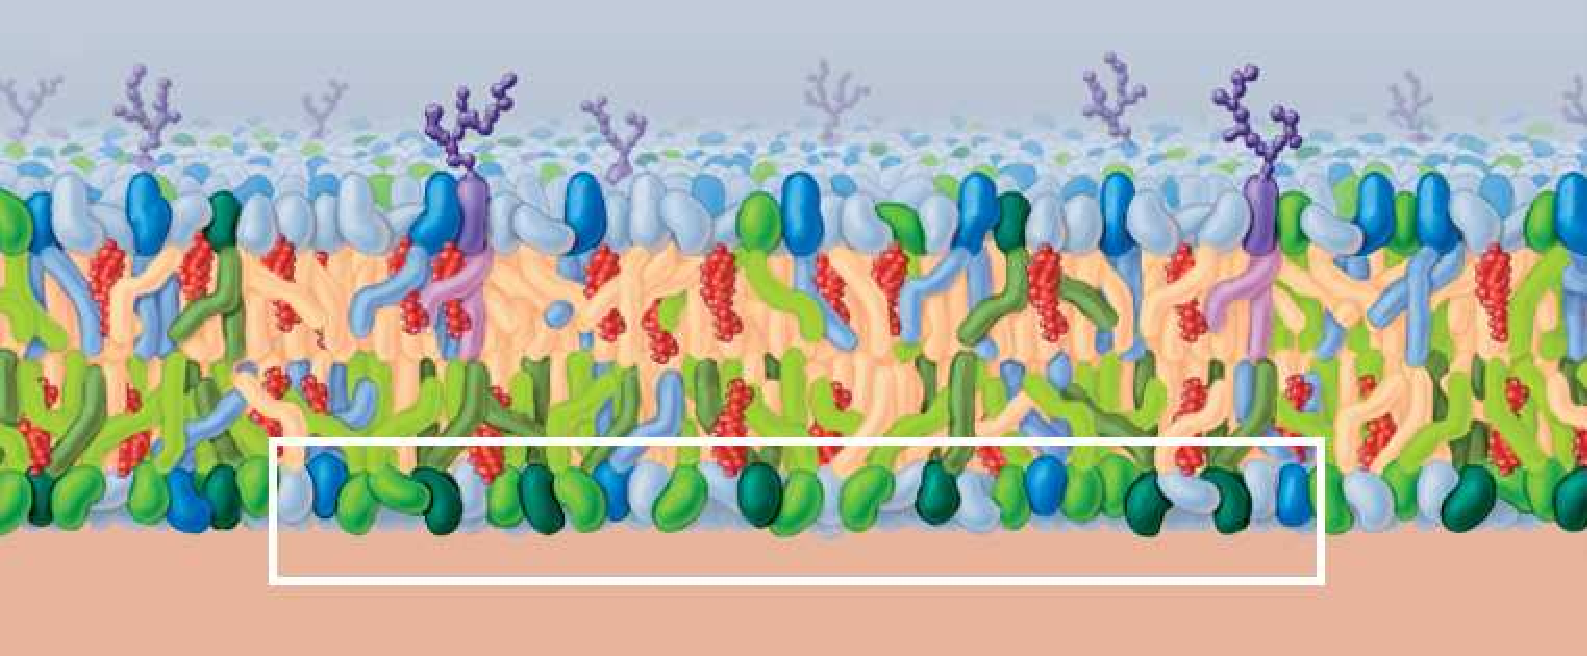
\includegraphics[scale = 0.54]{../figures/membrane_selected.pdf}
\end{center}
\caption[Cell membrane structure]{Cell membrane structure (adapted from \cite{Pollard2008}). Top surface (the outer leaflet of the membrane) and the bottom surface (the inner leaflet of the membrane) constitute the membrane bilayer structure. The space between the top and the bottom surfaces is the bilayer interior. White rectangle shows a slice of the inner leaflet with the lipid head groups, which is considered further in the thesis.}
\label{fig:membrane_from_book}
\end{figure}

Together with its complicated structure (Fig. \ref{fig:membrane_from_book}), the membrane has a wide range of biological functions. As an interface the membrane contains receptors which receive information from the extracellular environment. Various external molecules can be engulfed by the cell through the membrane by means of various processes, such as endocytosis, phagocytosis etc \cite{Doherty2009}. Cell growth and proliferation lead to the increase of the membrane area. Many signaling pathways are initiated on the membrane by activated membrane receptors and further propagate into the cell. All of these processes require the recruitment of various protein molecules to the cell membrane, as well as the alteration of the membrane composition. On the molecular level these processes are governed by physical laws. The well known example is the physical diffusion. The diffusion occurs everywhere in the cell and is particularly significant for the membrane organization \cite{Tocanne1989}. However, an impact of other physical principles involved in the membrane functionality is yet not well understood.

Electrostatics along with the diffusion is vital for the cell functions. The reason is that, firstly, most of the intracellular proteins, as sequences of amino acids, have parts with charged residues. Secondly, the cell cytoplasm consists of positively and negatively charged ions, that constitute its electrolytic nature \cite{Voets1999}. Finally, the cell membrane is also charged and interacts with cytoplasmic proteins and ions by means of electrostatic forces \cite{McLaughlin2005a}.

This thesis represents an investigation of the role of electrostatic interactions in the membrane lateral dynamics. Particularly, I concentrate on the lateral dynamics of membrane lipids and peripheral cytoplasmic proteins recruited and bound to the membrane.

I begin this introductory chapter with the description of the membrane composition and electrostatic properties. Next, I provide an overview of the electrostatic membrane adsorption of peripheral proteins and describe the structure of a specific type of these proteins -- proteins with polybasic domains. Then, I introduce the experimental and the theoretical data available on the membrane lateral dynamics. Finally, I define the goals of the thesis and provide its structure.

\section{Membrane composition and properties}

The major components of the cell membrane are various lipid species. Lipids are small amphiphilic molecules consisting of hydrophobic (tails) and hydrophilic (head groups) parts. The human body consists of several kg of membrane lipids with a total surface of about 0.4 km$^2$/kg and the plasma membrane of one eucariotic cell contains about 10$^{10}$ lipids, organized in a bilayer \cite{Heimburg2007}. The bilayer of the cell membrane is a stable structure, consisting of the bilayer interior, the inner (intracellular, in contact with the cell cytoplasm) and the outer (extracellular, in contact with the extracellular environment) leaflets (Fig. \ref{fig:membrane_from_book}). The interior of the bilayer is filled with the hydrophobic lipid tails, while the surfaces of the leaflets are populated with the hydrophilic lipid head groups. The outer leaflet of the membrane is generally neutral and does not significantly contribute to the membrane electrostatic properties. In contrast, the inner cytoplasmic leaflet, which consists of about 20--40\% of negatively charged lipids \cite{Kiessling2009}, constitutes the electrostatic nature of the membrane. The lipids, that create the charge of the inner membrane leaflet, belong to the class of lipids called phosphoglycerides (or phospholipids).

\subsection{Phospholipid head group structure and charge}

\label{phospholipids}

Phospholipids is the most abundant class of the membrane lipids. As all other lipids, a phospholipid has a hydrophobic tail connected (through glycerol and a phosphoric acid) to a head group (Fig. \ref{fig:phospholipids}, A). While the tail usually consists of two fatty acids, the head group has a more complicated structure (Fig. \ref{fig:phospholipids}, B).

\begin{figure}[!ht]
%\centering
%\scalebox{1.0}[1.0]
\begin{center}
  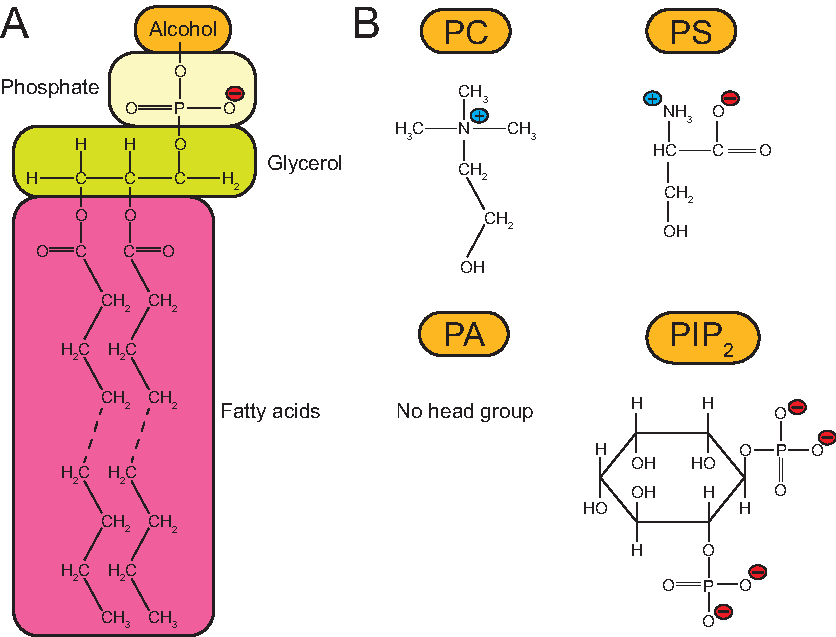
\includegraphics[scale=0.98]{../figures/Phospholipids.pdf}
\end{center}
 \caption[Phospholipid structures]{Phospholipid structures (adapted from \cite{Pollard2008}). A, Schematic structure of a phospholipid; B, Structures of the head group alcohols of different phospholipids.}
\label{fig:phospholipids}
\end{figure}

The main difference between phospholipids is the structure of the alcohol attached to the phosphate. Here I consider four types of membrane phospholipids with different structures of their alcohols: PC -- phosphatidylcholine (choline alcohol), PS -- phosphatidylserine (serine alcohol), PA -- phosphatidic acid (no head group) and PIP$_2$ -- phosphatidylinositol 4,5-bisphosphate (with inositol ring) (Fig. \ref{fig:phospholipids}, B). Since glycerol is neutral and the phosphate is always negatively charged (charge -1 in electron charge units), the net charge of the head group (together with the phosphate) is defined by the structure of the alcohol. For example, the net head group charge of a PC lipid is 0, since the positive charge of its alcohol neutralizes the negative charge of a phosphate group. In contrast, PS lipid has an additional negative charge in its alcohol, thus the net charge of its head group is -1. PA lipid, due to the absence of the alcohol, has only one negative charge in a phosphate group, thus its net charge is -1. PIP$_2$ has an unusual structure, which makes it a part of the class of lipids called phosphoinositides. The net head group charges of phosphoinositides are generally more negative than charges of other phospholipids. PIP$_2$ has 4 negative charges on the inositol ring, thus the maximum PIP$_2$ charge can be -5 (together with the phosphate charge). However, in the relevant biological conditions due to binding of cytoplasmic ions, such as K$^+$ or H$^+$, the charge of PIP$_2$ can be -3, -4 or -5 \cite{McLaughlin2002}.

\subsection{PIP$_2$ and other phosphoinositides}

\label{phosphoinositides}

Phosphoinositides constitute a small fraction (5-8\%) of the cell membrane lipids \cite{Cockcroft2001}. They have a specific inositol head group (the so-called inositol ring -- Fig. \ref{fig:phospholipids}, B). The main distinctive feature of the inositol ring is that it has 6 nodes (positions) and can be phosphorylated at them, allowing different structures and consequently different net charges of the ring. Phosphoinositides play a major role in the vital cell processes, such as signaling pathways, exo- and endocytosyses and others. The predecessor of all phosphoinositides is phosphatidylinositol (PI). PI undergoes changes of its structure through phosphorylation and dephosphorylation cycles by specific PI kinases and phosphatases, providing other phosphoinositides (Fig. \ref{fig:PI_cycle2}).

\begin{figure}[!ht]
%\centering
%\scalebox{1.0}[1.0]
\begin{center}
  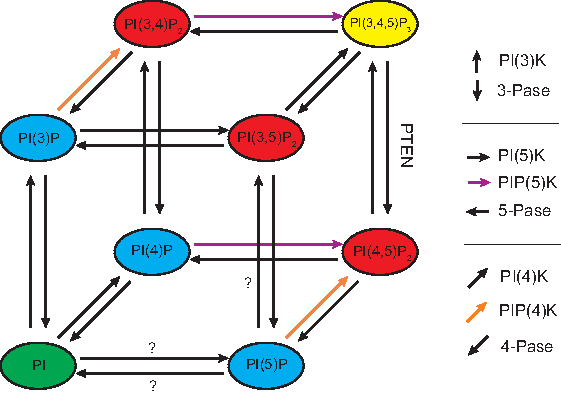
\includegraphics[scale=1.2]{../figures/PI_cycle2.pdf}
\end{center}
 \caption[Diagram of phoshoinositides regulation]{Diagram of phoshoinositides regulation. Phosphoinositides are shown in colored ovals. The enzymes involved in the phosphoinositides regulation are shown with arrows of different colors and different directions. Unknown enzymes are shown with ``?''.}
\label{fig:PI_cycle2}
\end{figure}

PIP$_2$ phosphoinositide, which comprises only about 1\% of the cytoplasmic leaflet of the plasma membrane, has a large number of functions, such as a source of three major second messengers (DAG, IP$_3$ and PIP$_3$), one of the main components of both exo- and endocytosis, an anchor for the peripheral membrane proteins and many others \cite{Martin2001,Toker1998,Lee1995,Nebl2000}. PIP$_2$ biophysical properties distinguish it from all other non-inositial membrane components. In addition to its strongly negative charge (-4), described in the previous chapter, PIP$_2$ headgroup may also protrude much further in the aqueous phase than a typical phospholipid \cite{Li2009}. Due to these distinguishing characteristic PIP$_2$ is able to interact with cytoplasmic proteins with high affinity, especially with strongly positively charged parts of proteins.

\section{Electrostatics of the membrane adsorption}

\label{adsorption_introduction0}

Electrostatic properties of the membrane lipids described above play a crucial role in the membrane binding of the peripheral proteins. Peripheral membrane proteins are able to temporally attach to the membrane by insertion of a covalent lipid modifications in it \cite{Fivaz2003}. A covalent lipid modification is a covalent addition of a fatty acid to one of the protein ends. During the membrane binding the lipid modification is hydophobically inserted to the lipid bilayer and due to the hydrophobic effect the total structure stabilizes. However, in many cases the hydrophobic insertion of a lipid modification is not sufficient to keep a protein attached \cite{McLaughlin1995}. In these cases electrostatic interactions of the proteins with membrane negatively charged lipids can effectively facilitate the binding \cite{Wang2001,Arbuzova2000}. Remarkably, several highly important signaling proteins, such as Ras small GTPases, phosphatase PTEN, and actin regulators WASP and MARCKS as well as nonreceptor tyrosine kinase Src, along with other binding mechanisms, bind to the membrane using a sequence of positively charged residues in their structure, which is called a polybasic domain (PD) \cite{Hancock1990,Murray1998,Fivaz2003,McLaughlin1995,Wang2002,Das2003}. It has been shown experimentally that the PD contributes approximately the same amount of energy to the membrane binding (for 2:1 PC/PS membrane) as the hydophobic insertion of the lipid modification \cite{McLaughlin1995}. These examples show that the PD is essential for binding of various signaling proteins to the negatively charged inner leaflet of the cell membrane.

\subsection{Protein polybasic domain}

\label{proteins_polybasic_domain}

To provide an example of a PD, I concentrate here on the PD of MARCKS protein (151-175), since it has a common structure and has been extensively studied and well described. The structure of the domain is presented in Fig. \ref{fig:PD}, taken from \cite{Wang2001}. The PD of MARCKS protein consists of 13 basic residues that interact electrostatically with negatively charged membrane lipids. The main contribution to the electrostatic PD binding is provided by the first 5 basic residues \cite{Denisov1998} (Fig. \ref{fig:PD}, shown as blue plus signs at the left side of the domain).
\begin{figure}[!ht]
%\centering
%\scalebox{1.0}[1.0]
\begin{center}
  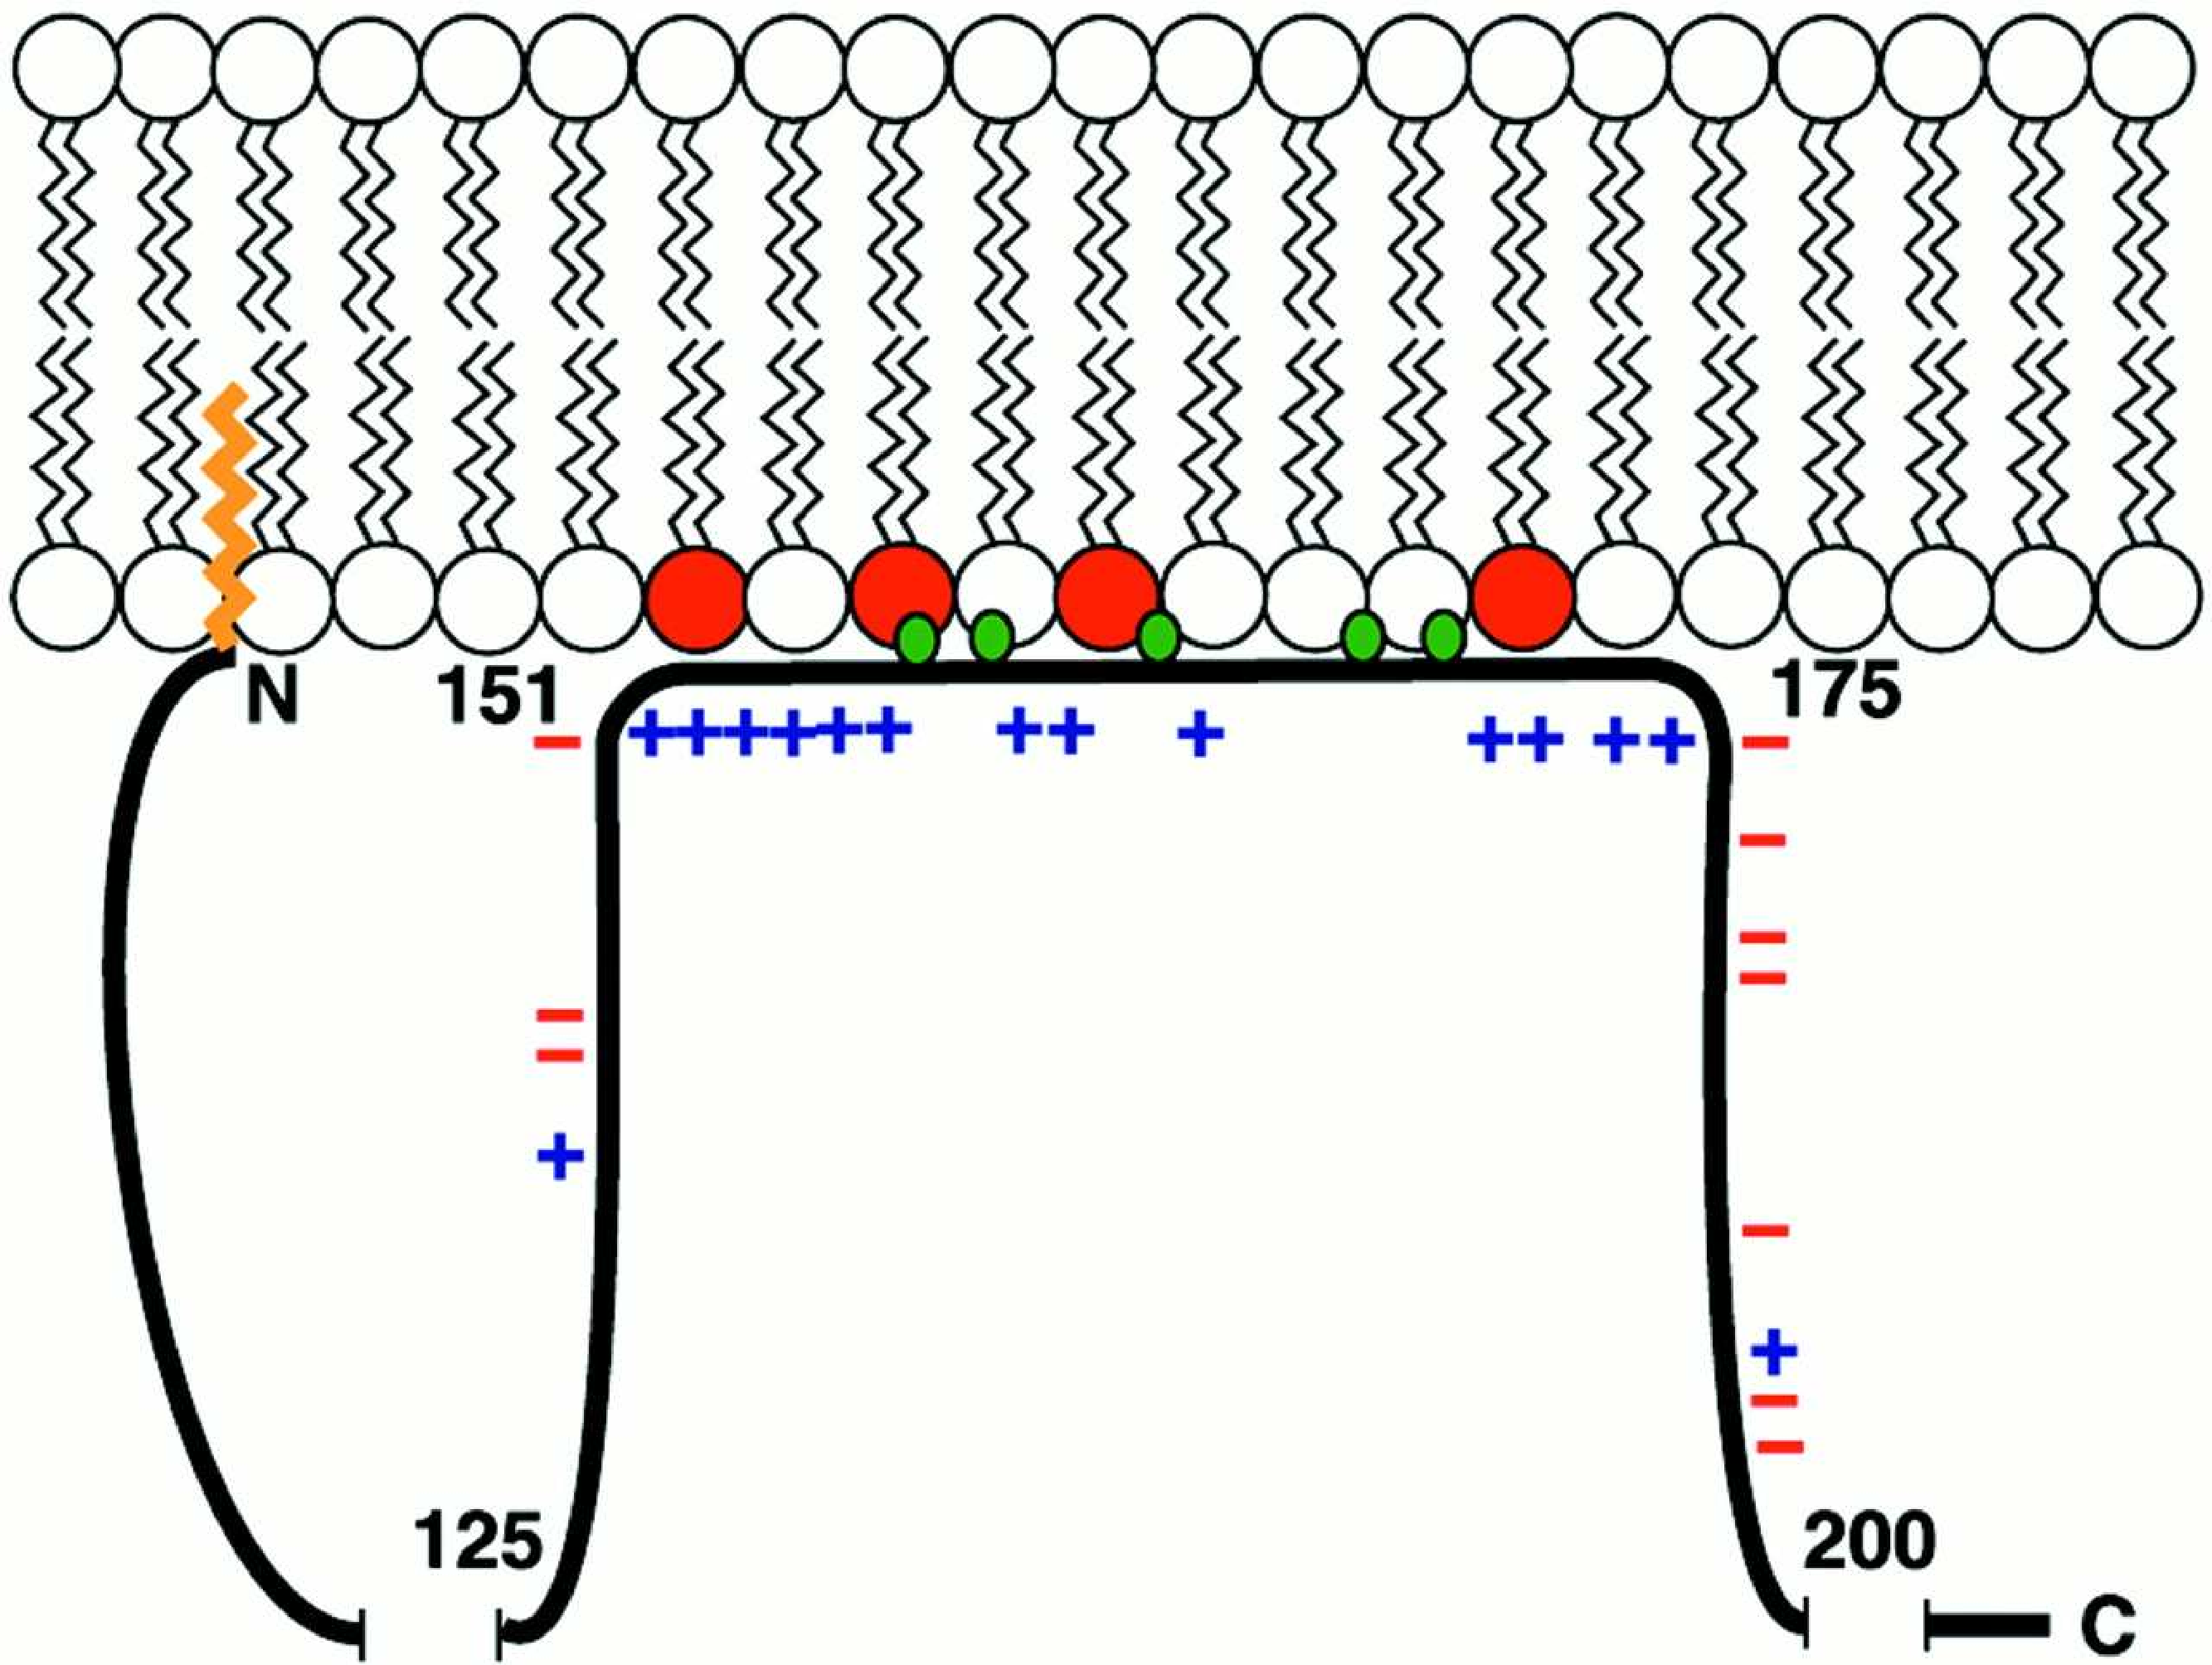
\includegraphics[scale=0.25]{../figures/PD.pdf}
\end{center}
 \caption[Schematic representation of MARCKS interacting with the membrane]{Schematic representation of MARCKS interacting with the membrane (from \cite{Wang2001}). The PD is a black line between the 151$^{\text{th}}$ and the 175$^{\text{th}}$ protein residues. The lipid modification inserted in the membrane bilayer is shown in orange. The positively charged residues of the PD are shown as blue plus signs. Negatively charged membrane lipids (PS, PA, PIP$_2$) are shown as red circles, neutral lipids (PC) are shown as white circles. 5 aromatic residues are shown in green.}
\label{fig:PD}
\end{figure}
Additionally, there are 5 aromatic residues that also contribute to the protein membrane binding (Fig. \ref{fig:PD}, shown in green). These aromatic residues during binding penetrate the polar head group region of the membrane \cite{Arbuzova2000}. However, the energy of their interactions with the membrane is insignificant, compared to the contribution from the PD and the lipid modification \cite{Wang2002,McLaughlin1995}. Electron paramagnetic resonance \cite{Qin1996} and circular dichroism \cite{Wang2001} studies indicated that MARCKS PD is unstructured and elongated when bound to a membrane.



\subsection{Membrane adsorption of PDs and lipid demixing}

\label{adsorption_introduction}

Electrostatic adsorption of proteins to the membrane has been a subject of many scientific investigations. A lot of experimental work has been done to \mbox{measure} membrane adsorption isotherms and binding constants of peripheral membrane proteins with PDs, as well as small peptides with characteristic structure, corresponding to the structure of the PD \cite{Heimburg1999,Murray1998,Denisov1998,Ben-Tal1996}. To describe the mechanism of electrostatic adsorption of the PD to the membrane in detail a large number of computational models have been developed. The structures of the PDs considered in the models vary from simple charged objects (e.g. a sphere or a cylinder) \cite{Tzlil2005, Mbamala2005, Heimburg1999} to more detailed and biologically relevant molecular representations of the PDs \cite{Denisov1998,Ben-Tal1996,Murray1998,Tzlil2008}. As a result of these studies a new phenomenon of lipid demixing (or sequestration) upon electrostatic protein adsorption has been discovered experimentally and described theoretically \cite{Heimburg1999,Wang2002,Golebiewska2006,Gambhir2004,Wang2004,May2000,Haleva2004}. Lipid demixing represents a redistribution of lipids in the vicinity of the charged adsorbed molecule (PD). Negatively charged lipids, such as PS, PA or PIP$_2$ tend to aggregate around the positively charged parts of the adsorbed PD. Thus, the \mbox{concentration} of negatively charged lipids in the vicinity of the PD becomes higher than in the rest of the membrane. Since the area of the membrane with higher density of negatively charged lipids is more attractive for other proteins with PDs, lipid demixing can potentially give rise \cite{Denisov1998,May2000,Mbamala2005} to formation of recently characterized membrane microdomains \cite{Day2009,Goryachev2008}. Interestingly, it has been shown that, upon lipid demixing in ternary (PC/PS/PIP$_2$) membranes, mainly PIP$_2$ lipids, due to their strong negative charge -4, relocate to the area of adsorption, displacing neutral PC and monovalent PS lipids \cite{Wang2002,Golebiewska2006,Gambhir2004,Wang2004,Haleva2004}.

\section{Protein and lipid membrane dynamics}

\label{protein_lipid_dynamics_intoduction}

Between adsorption to and desorption of any protein from the membrane there is a finite time interval, during which the protein remains bound to the membrane. The average time interval of the protein being bound to the membrane is called the association time and is defined by various factors (e.g. the energy of binding, etc.). The range of associations times varies from sub-seconds to several hours \cite{Fivaz2003}. During the association time the proteins are not static, but generally undergo lateral diffusion on the membrane.

Lateral dynamics of proteins on the biological membranes has been extensively studied in the last decades \cite{Singer1972,Saffman1975,Axelrod1983}. The development of several biophysical methods, such as fluorescence recovery after photobleaching (FRAP) and fluorescence correlation spectroscopy (FCS) \cite{Chen2006} allowed to visualize lipids and proteins on the membrane and explore their diffusive properties. Introduction of artificial membranes, such as supported phospholipid bilayers \cite{Tamm1985}, enabled to perform experiments in a well-controlled \emph{in vitro} environment. The experiments showed that peripheral membrane proteins, such as GPI-anchored proteins and lipid-specific antibodies, are generally 2--8 times slower than lipids \cite{Zhang1991, Tamm1988, Stefl2009}.

It also became clear that electrostatic interactions between proteins and membrane lipids determine lipid lateral mobility. For example, it has been shown that Annexin IV, adsorbed to the surface of a PG (charge -1)/PC bilayer, due to electrostatic interactions, is an important determinant of lipid lateral mobility \cite{Gilmanshin1994}. As described in section \ref{adsorption_introduction}, PIP$_2$ performs a rapid demixing upon protein membrane adsorption and is strongly sequestered by positively charged residues of the PD. This can be a reason of an experimentally measured slower ($D=0.8\pm0.2$ $\mu$m$^{2}$/s) PIP$_2$ diffusion on the inner leaflet of fibroblasts and epithelial cells compared to its diffusion measured within cellular blebs and artificial phospholipid membranes ($D=2.5-3.3$ $\mu$m$^{2}$/s). This finding is also in agreement with other results obtained for both PIP$_2$ and PIP$_3$ \cite{Haugh2000, Yaradanakul2007}.

The application of the fluorescent protein techniques enabled the \emph{in vivo} analysis of the dynamics of proteins on the inner leaflet of the plasma membrane. These analyses demonstrated that under physiological conditions (20--40\% of monovalent lipids and $<$1\% of PIP$_2$) diffusion coefficients of proteins attached by a lipid modification and a polybasic domain are similar to those of other peripheral membrane proteins \cite{Fivaz2003}. For example, the inactive (tightly folded) conformation of Src with the PD was shown to diffuse with the mobility $D=0.57$ $\mu$m$^{2}$/s \cite{Shvartsman2007}, however, other members of Src family, devoid of polybasic domain, were found to have similar mobilities: $D=0.1-0.6$ $\mu$m$^{2}$/s \cite{Lu2008, Larson2005, Frick2007, Pyenta2003,Zimmermann2010}. Analogously, small GTPase KRas with the pronounced PD (+7) was found to diffuse with the mobility $D=0.2-0.35$ $\mu$m$^{2}$/s \cite{Lu2008, Pyenta2003, Niv2002}, which is close to that of HRas ($D=0.35-0.5$ $\mu$m$^{2}$/s) \cite{Niv2002} that has no PD.

Considerably less, however, is known about the influence of different concentrations of negatively charged lipids on the lateral dynamics of proteins with the PDs. Only a few \emph{in vitro} studies revealed the significant changes of the PD diffusion coefficients upon varying the concentrations of anionic lipids. For example, Golebiewska et al. \cite{Golebiewska2006} demonstrated that Lys-13, a peptide mimicking the PD of MARCKS protein, diffuses slower on GUVs containing 1\% of PIP$_2$ than on vesicles consisting only of neutral PC and monovalent PS (-1) lipids.

\section{Computational modeling of protein and lipid membrane dynamics}

\label{protein_lipid_dynamics_modeling}

Computational modeling has been playing a considerable role in characterization of various aspects of protein diffusion on biological membranes \cite{Saxton1989, Sung2009, Haugh2009, Gil1998}. Electrostatic interactions between lipids and proteins have also received significant theoretical attention. However, most of it has been focused on the adsorption-desorption dynamics of proteins and the associated demixing of negatively charged lipids (see chapter \ref{adsorption_introduction}), while the contribution of electrostatic interactions to the lateral dynamics of adsorbed proteins remained largely unexplored. Only a few studies took this phenomenon into account.

Hinderliter et al. \cite{Hinderliter2001} performed Monte-Carlo simulations of multiple proteins on a lattice and, in addition to adsorption and desorption, introduced protein diffusion. However, how electrostatic interaction of proteins with underlying lipids contributed to the protein lateral dynamics was not considered in detail. 

Recently, Khelashvili et al. \cite{Khelashvili2008} developed a hybrid (Monte-Carlo simulations coupled to the mean-field approximation) approach in which lateral dynamics of a single poly-lysine peptide and the surrounding lipid was simulated by alternation of random peptide moves and lipid relaxation in accordance with Cahn-Hillard equation. However, due to the absence of explicit thermal fluctuations in the lipid subsystem, lipids did not possess lateral dynamics independent of that of the peptide.

\section{Thesis objectives and structure}

As described above (sections \ref{protein_lipid_dynamics_intoduction} and \ref{protein_lipid_dynamics_modeling}), the electrostatic contribution to the lateral dynamics of proteins and consequent dynamics of lipids in biological membranes has not been sufficiently studied and the developed modeling tools describe this phenomenon only partially. The goal of this thesis is to uncover new insights into the membrane lateral dynamics by constructing new modeling tools that will be able to describe the electrostatic impact on the membrane dynamics in details. The main objective of the thesis is:

\begin{quotation}
\begin{spacing}{1.0}
\emph{To extend the understanding of the electrostatic contribution to the membrane lateral dynamics of proteins and lipids by means of novel computational modeling tools.}
\end{spacing}
\end{quotation}

\vspace{-0.23in}

To fulfill this objective, first, I develop a discrete computational model that simulates the behavior of a protein bound to the negatively charged cell membrane. This is a Monte-Carlo simulation model based on the Metropolis algorithm. I describe the details of the model development and implementation in the chapter \ref{Monte_Carlo_model_description}. To test and validate the model I simulate the lipid and protein dynamics on the membrane with the uniform composition. The results of the discrete model obtained on the uniform membrane are provided at the end of chapter \ref{Monte_Carlo_model_description}.

Second, I use the Monte-Carlo model described in chapter \ref{Monte_Carlo_model_description} to better understand the influence of the distribution of negatively charged lipids on protein lateral dynamics. Particularly, I make the concentrations of lipids in the membrane non-uniform and run the simulations of the protein diffusion. These simulations are described in the chapter \ref{non_uniform_membrane}.

Thirdly, in chapter \ref{continuous_model_description}, based on the results of the Monte-Carlo simulation model and the thermodynamical approach, I construct a novel continuous model of protein and lipid lateral membrane dynamics. I also discuss the limitations of the continuous model and its advantages  over the discrete Monte-Carlo simulation model. One of the main advantages of the continuous model is that it allows one to study electrostatic effects on the membrane at larger (several micrometers) scales, as compared to the maximal size (the order of 100 nm) of the membrane domain in the Monte-Carlo simulation model.

In chapter \ref{comparison_chapter} I compare the results obtained in the continuous model with the results of Monte-Carlo simulations for the non-uniform membrane compositions (with lipid gradients).

Finally, I conclude the thesis by explaining how its main objective has been fulfilled and what contributions to the science my work has made. I also provide possible future directions of the research where the developed computational tools can be particularly useful.